\chapter{Vyhodnotenie}\label{ch:evaluation}


Táto kapitola sa zaoberá vyhodnotením navrhnutého kvantového generátora náhodných čísel (QRNG) z hľadiska kvality generovanej náhodnosti, stability výstupu a jeho kryptografickej použiteľnosti. Vyhodnotenie je založené na spracovaní dát získaných z kvantového zariadenia a ich následnej štatistickej analýze pomocou viacerých metód.


\section{Metódy merania a spracovania dát}


Meranie náhodnosti bolo realizované na základe dát získaných z kvantového zariadenia vo forme jednotlivých meraní (tzv. \textit{shots}).
Každé meranie obsahovalo výsledky merania viacerých qubitov, ktoré boli následne spracované do binárnej reprezentácie.


Z nameraných dát boli vytvorené dvojice Bellových párov qubitov, pričom každá dvojica reprezentovala jeden výsledný bit.
Mapovanie Bellových párov na klasické bity bolo definované nasledovne:


\begin{itemize}

  \item stav $(0,0)$ bol mapovaný na bit 0,

  \item stav $(1,1)$ bol mapovaný na bit 1,

  \item stav $(0,1)$ bol mapovaný na bit 1,

  \item stav $(1,0)$ bol mapovaný na bit 0.

\end{itemize}


Takto získané bity boli zoradené do bitových reťazcov pre jednotlivé merania a následne spojené do jedného dlhého bitového toku. Tento tok predstavuje základný vstup pre všetky ďalšie analýzy.


Na zníženie biasu a elimináciu možných korelácií spôsobených fyzikálnymi obmedzeniami kvantového zariadenia bola aplikovaná extrakcia entropie pomocou hashovacej funkcie MD5. Bitový tok bol rozdelený na bloky pevnej veľkosti, pričom každý blok bol transformovaný hashovacou funkciou a výsledné bity boli použité ako nový, upravený bitový tok. Tento proces zvyšuje uniformitu rozdelenia a znižuje potenciálne štrukturálne závislosti.


\section{Metódy vyhodnotenia}


Vyhodnotenie kvality generovaného bitového toku bolo realizované kombináciou viacerých prístupov, ktoré zahŕňajú štatistické testy, analýzu distribúcie, testy predikovateľnosti a praktické overenie generovania náhodných hodnôt.


\subsection{Analýza distribúcie bitov}


Základným krokom vyhodnotenia bolo overenie rovnomernosti rozdelenia núl a jednotiek. Bitový tok bol rozdelený na viacero segmentov, pričom pre každý segment bol vypočítaný počet núl, počet jednotiek a ich relatívne zastúpenie.


Pre každý segment boli určené hodnoty:

\begin{itemize}

  \item $p_0$ – pravdepodobnosť výskytu nuly,

  \item $p_1$ – pravdepodobnosť výskytu jednotky,

  \item bias – absolútna odchýlka od ideálnej hodnoty $0{,}5$.

\end{itemize}


Táto analýza umožňuje sledovať stabilitu generátora v čase a identifikovať prípadné lokálne odchýlky od ideálneho náhodného správania.


\subsection{NIST testy náhodnosti}


Na overenie náhodnosti bitového toku boli implementované testy inšpirované metodikou NIST Statistical Test Suite:


\begin{itemize}

  \item \textbf{Frequency test (monobit test)} – overuje, či je počet núl a jednotiek vyvážený,

  \item \textbf{Runs test} – analyzuje počet a dĺžku behov rovnakých bitov,

  \item \textbf{Cumulative sums test} – sleduje maximálnu odchýlku kumulatívneho súčtu od očakávanej hodnoty.

\end{itemize}


Výsledkom každého testu je $p$-hodnota, ktorá vyjadruje pravdepodobnosť, že analyzovaný bitový tok pochádza z náhodného zdroja. Hodnoty nižšie ako zvolená hladina významnosti indikujú odchýlku od náhodnosti.


\subsection{Test predikovateľnosti (Next-bit test)}


Dôležitou súčasťou vyhodnotenia bola analýza predikovateľnosti bitového toku. Bol použitý tzv. next-bit test, ktorého cieľom je overiť, či je možné predpovedať nasledujúci bit na základe predchádzajúcich bitov.


Bitový tok bol transformovaný na dataset, kde vstup predstavuje pevne dané okno predchádzajúcich bitov a výstup nasledujúci bit. Na predikciu bol použitý model logistickej regresie so štandardizáciou vstupných dát.


Na zabezpečenie korektného vyhodnotenia bola použitá metóda časovo usporiadaných validačných množín (tzv. expanding window cross-validation), ktorá zabraňuje úniku informácií z budúcnosti do minulosti.


Výkonnosť modelu bola hodnotená pomocou metrík:

\begin{itemize}

  \item accuracy,

  \item balanced accuracy,

  \item ROC AUC,

  \item log-loss.

\end{itemize}


Na overenie štatistickej významnosti výsledkov bol použitý binomický test, ktorý porovnáva úspešnosť modelu s náhodným hádaním.


\subsection{Markovov test}


Ako doplnková metóda bol použitý Markovov model, ktorý analyzuje závislosť medzi po sebe idúcimi bitmi. Model odhaduje pravdepodobnosť nasledujúceho bitu na základe konkrétneho vzoru predchádzajúcich bitov.


Vyhodnotenie prebiehalo rozdelením dát na trénovaciu a testovaciu množinu, pričom výsledná presnosť a $p$-hodnota poskytujú informáciu o existencii lokálnych závislostí v bitovom toku.


\subsection{Test distribúcie generovaných hodnôt}


Na praktické overenie použiteľnosti generátora boli z bitového toku generované čísla v diskrétnych intervaloch, napríklad simuláciou hodu kockou alebo generovaním 4-bitových hodnôt.


Použitá bola metóda \textit{rejection sampling}, ktorá zabezpečuje rovnomerné rozdelenie výsledkov aj v prípade, že rozsah hodnôt nie je mocninou dvojky. Následne boli analyzované frekvencie jednotlivých hodnôt a porovnané s ideálnym rovnomerným rozdelením.


\section{Vyhodnotenie výsledkov}


Na základe vykonaných analýz možno konštatovať, že generovaný bitový tok vykazuje dobré štatistické vlastnosti.
Taktiež sa nám úspešne podarilo experimentálne overiť možnosť existencie generátora náhodných čísel založeného na entropii kvantového počítača.
Rozdelenie núl a jednotiek je vo väčšine prípadov blízke ideálnemu pomeru, pričom odchýlky sú v rámci očakávaných štatistických limitov.


Výsledky NIST testov nepreukázali systematické porušenie náhodnosti, pričom $p$-hodnoty sa pohybovali v akceptovateľných intervaloch.
Podobne aj rozšírené testy neodhalili výrazné anomálie.


Analýza predikovateľnosti ukázala, že model logistickej regresie nedokáže predpovedať nasledujúci bit s presnosťou významne vyššou než náhodné hádanie.
Tento výsledok je podporený aj hodnotami $p$-hodnôt z binomického testu, ktoré neindikujú štatisticky významnú predikovateľnosť.


Markovov test taktiež nepreukázal významnú závislosť medzi po sebe idúcimi bitmi, čo naznačuje absenciu jednoducho využiteľnej štruktúry.


%---------------------------------------------------------------------------------------------------------------------------------------------------------


\section{Návrh používateľského rozhrania}

Používateľské rozhranie systému bolo navrhované iteratívnym spôsobom, pričom bol kladený dôraz na postupné prototypovanie, neustále zlepšovanie a systematické overovanie návrhov priamo s používateľmi.
Tento prístup umožnil rýchlo a efektívne reagovať na zistené nedostatky, optimalizovať interakciu a zabezpečiť, aby finálne riešenie bolo intuitívne a zrozumiteľné.

Celý proces návrhu prebehol v rámci \textbf{dvoch prototypov}, pričom prvá iterácia bola ukončená formou systematického hodnotenia s reálnymi používateľmi.
Získané výsledky poskytli cenné podklady a spätnú väzbu, ktoré boli následne využité pri návrhu a implementácii druhého prototypu.

Ako formálna metóda hodnotenia použiteľnosti bola zvolená štandardizovaná metodika \textit{System Usability Scale (SUS)}, ktorá umožňuje získať kvantitatívne skóre použiteľnosti systému.
Testovanie prebiehalo v súlade so štandardizovaným postupom a bolo doplnené o pozorovanie a nahrávanie správania používateľov počas prechádzania vopred definovaných používateľských scenárov.


\subsection{Prvý prototyp a jeho overenie}

Prvý prototyp používateľského rozhrania bol vytvorený ako základný statický prototyp zameraný na overenie hlavných konceptov návrhu v dizajnérskom nástroji Figma.
Jeho cieľom bolo overiť správnosť návrhu architektúry systému, zrozumiteľnosť pomenovania prvkov používateľského rozhrania a základné interakčné toky.
Úvodná obrazovka prvého prototypu je zobrazená na obr.~\ref{fig:prvyPrototyp}.

\begin{figure}[H]
  \centering
  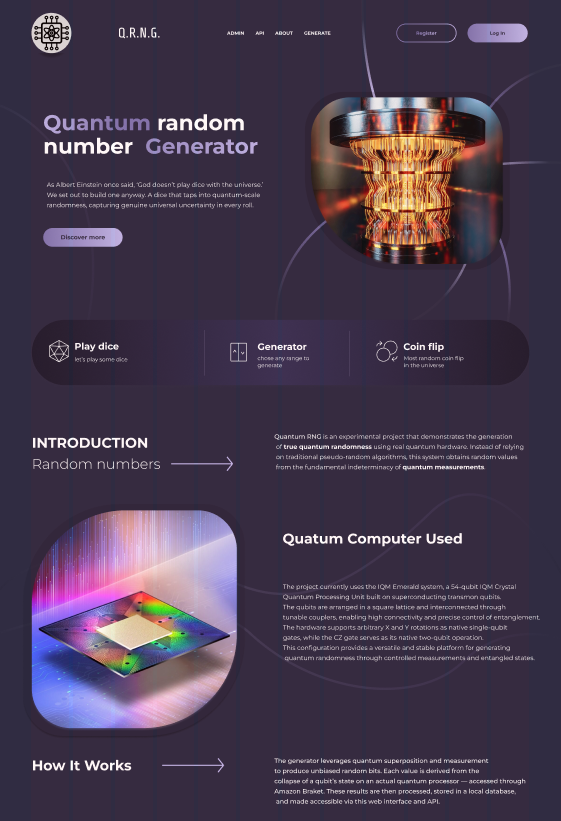
\includegraphics[width=0.55\textwidth]{images/prototypFigmaPrvy}
  \caption{Prvý prototyp vytvorený v nástroji Figma.}
  \label{fig:prvyPrototyp}
\end{figure}

Prototyp bol sprístupnený online vo forme interaktívneho prototypu\footnote{Figma interaktívny prototyp: \url{https://www.figma.com/board/CooSPjDeRGEgL9t9sCZlRs/UX3-PeterJas?node-id=0-1&p=f&t=BN1FOqv3hAIUkeSb-0}}.

Používateľské testovanie prvého prototypu bolo vykonané na vzorke piatich účastníkov.
Testovanie sa zameriavalo na úspešnosť plnenia definovaných úloh, čas potrebný na ich splnenie a subjektívne hodnotenie použiteľnosti rozhrania prostredníctvom SUS dotazníka.

Výsledky boli vyhodnotené pomocou metodiky SUS, pričom výsledná hodnota dosiahla skóre \textbf{49,5}.
Táto hodnota poukazuje na čiastočnú použiteľnosť rozhrania, avšak s viacerými identifikovanými problémami a výrazným priestorom na zlepšenie.

Pozorovanie používateľov počas prechádzania štyroch používateľských scenárov odhalilo viacero konkrétnych nedostatkov, na ktoré sa druhá iterácia zameriava.

\subsection{Druhý prototyp a jeho overenie}

Druhý prototyp už nepredstavuje iba návrhovú iteráciu, ale plnohodnotné funkčné riešenie, ktoré vzniklo na základe skúseností a spätnej väzby získanej z testovania prvého prototypu.
Na rozdiel od prvého prototypu je druhý prototyp implementovaný ako hotová webová aplikácia využívajúca technológie \textbf{HTML a CSS} na strane používateľského rozhrania a \textbf{Django backend} na strane serverovej logiky s databázou \textbf{SQLite}.
Vďaka tejto architektúre už systém nefunguje len ako simulácia, ale obsahuje reálne interakcie prepojené s databázou, ktorá zabezpečuje ukladanie a spracovanie údajov používateľov, históriu generovaných hodnôt a správu kvantových bitov.

Hlavná obrazovka aplikácie je znázornená na obr.~\ref{fig:druhyPrototypHome}.

\begin{figure}[H]
  \centering
  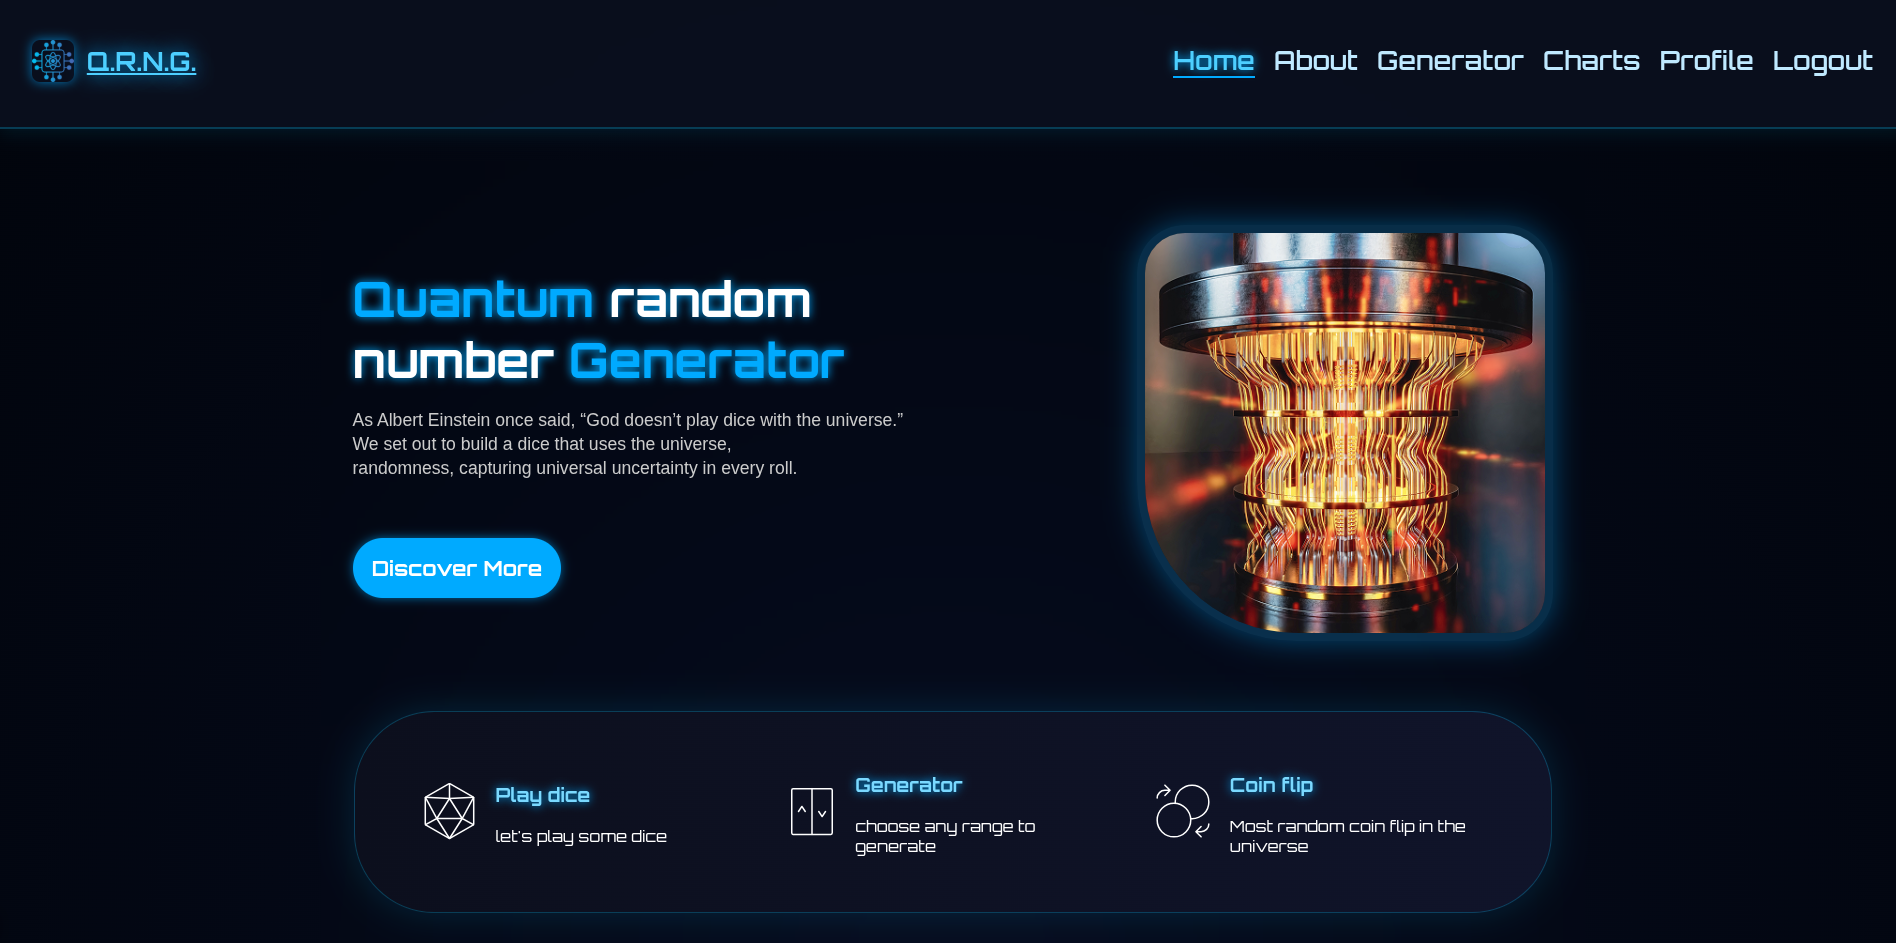
\includegraphics[width=0.9\textwidth]{images/prototypDruhy}
  \caption{Hlavná obrazovka druhého prototypu.}
  \label{fig:druhyPrototypHome}
\end{figure}



\subsection{Technologický základ aplikácie}

Finálne riešenie je implementované ako webová aplikácia postavená na frameworku \textbf{Django}, ktorý zabezpečuje serverovú logiku, správu používateľov a prístup k databáze.
Používateľské rozhranie je realizované pomocou technológií \textbf{HTML} a \textbf{CSS}, pričom jednotlivé stránky sú generované šablónovacím systémom Django (Jinja2-kompatibilné Django templates).

Ako databázové úložisko je použitá \textbf{SQLite}, ktorú Django poskytuje ako predvolenú relačnú databázu vhodnú pre vývojové a stredne zaťažené produkčné nasadenia.
Databáza uchováva viacero typov záznamov: kvantové výsledky meraní (\texttt{QuantumShotResult}), históriu generovania náhodných čísel pre každého používateľa (\texttt{RNGHistory}) a rozšírené profily používateľov (\texttt{Profile}).

Aplikácia využíva vlastný systém správy používateľov postavený nad vstavaným autentifikačným modulom Django.
Registrácia, prihlásenie a odhlásenie sú plne funkčné a integrované do navigácie aplikácie.

Smerovanie (routing) URL adries je definované v súbore \texttt{urls.py} a zahŕňa nasledujúce cesty:

\begin{itemize}
  \item \texttt{/} -- hlavná stránka aplikácie,
  \item \texttt{/coin/} -- generátor náhodného hodu mincou,
  \item \texttt{/dice/} -- generátor náhodného hodu kockou,
  \item \texttt{/generator/} -- všeobecný generátor náhodných čísel v zadanom rozsahu,
  \item \texttt{/charts/} -- štatistické grafy a vyhodnotenie generátora,
  \item \texttt{/about/} -- informačná stránka o projekte,
  \item \texttt{/administration/} -- administrátorský panel (prístup len pre administrátorov),
  \item \texttt{/accounts/profile/} -- profil prihláseného používateľa,
  \item \texttt{/accounts/history/} -- história generovania náhodných čísel.
\end{itemize}

\subsection{Generátory náhodných čísel}

Jadrom aplikácie sú tri moduly generovania náhodných čísel, každý prispôsobený odlišnému účelu.
Všetky tri moduly čerpajú náhodnosť z rovnakého zdroja: triedy \texttt{QuantumDBStream}, ktorá postupne číta bity uložené v databáze z kvantových meraní a vydáva ich metódou \texttt{get\_random(min, max)}.
Táto metóda implementuje algoritmus \textit{rejection sampling}, ktorý zaručuje rovnomerné rozdelenie hodnôt aj v prípadoch, keď požadovaný rozsah nie je mocninou čísla 2.

\subsubsection{Hod mincou}

Modul hodu mincou (\texttt{/coin/}) umožňuje používateľovi simulovať hod jednou alebo viacerými mincami súčasne.
Používateľ zadá počet mincí (od 1 do 6) a po odoslaní formulára aplikácia vygeneruje pre každú mincu hodnotu v rozsahu $\langle 1, 2 \rangle$, pričom hodnota 1 je interpretovaná ako \textit{Heads} (orol) a hodnota 2 ako \textit{Tails} (písmo).
Výsledky sú zobrazené ako karty s textovým popisom, ako je znázornené na obr.~\ref{fig:coinPage}.

\begin{figure}[H]
  \centering
  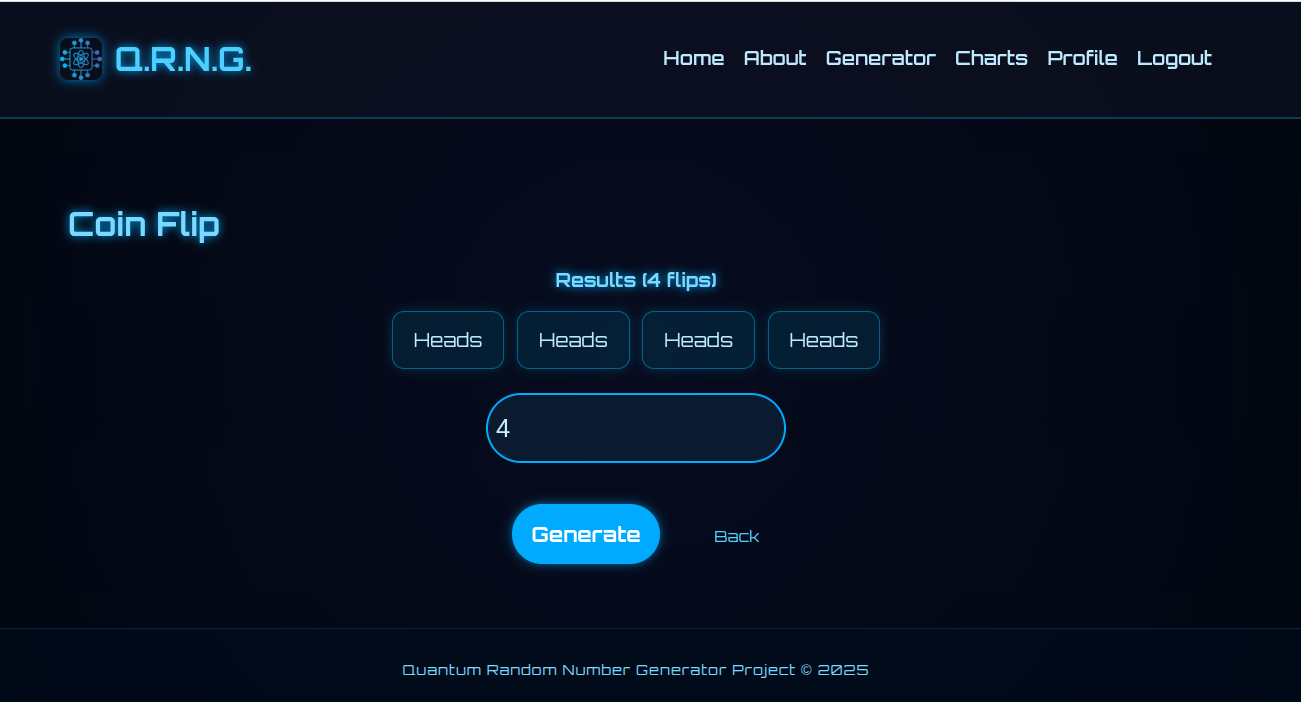
\includegraphics[width=0.9\textwidth]{images/coinHeadsTails}
  \caption{Stránka hodu mincou s výsledkami.}
  \label{fig:coinPage}
\end{figure}

\subsubsection{Hod kockou}

Modul hodu kockou (\texttt{/dice/}) patrí k najbohatšie vybaveným generátorom v aplikácii.
Používateľ si môže zvoliť typ kocky z ôsmich dostupných variantov: \textbf{d4, d6, d8, d10, d12, d20, d50 a d100}.
Táto škála pokrýva štandardné herné kocky používané v stolných hrách a roleplaying hrách, no zároveň rozširuje ponuku o menej bežné varianty (d50, d100), ktoré bývajú užitočné pri stochastických simuláciách.
Okrem typu kocky si používateľ zvolí aj počet hodov (od 1 do 6), ktoré sa vykonajú naraz.
Výsledky sú zobrazené ako skupiny číselných kariet, ako je znázornené na obr.~\ref{fig:dicePage}.

\begin{figure}[H]
  \centering
  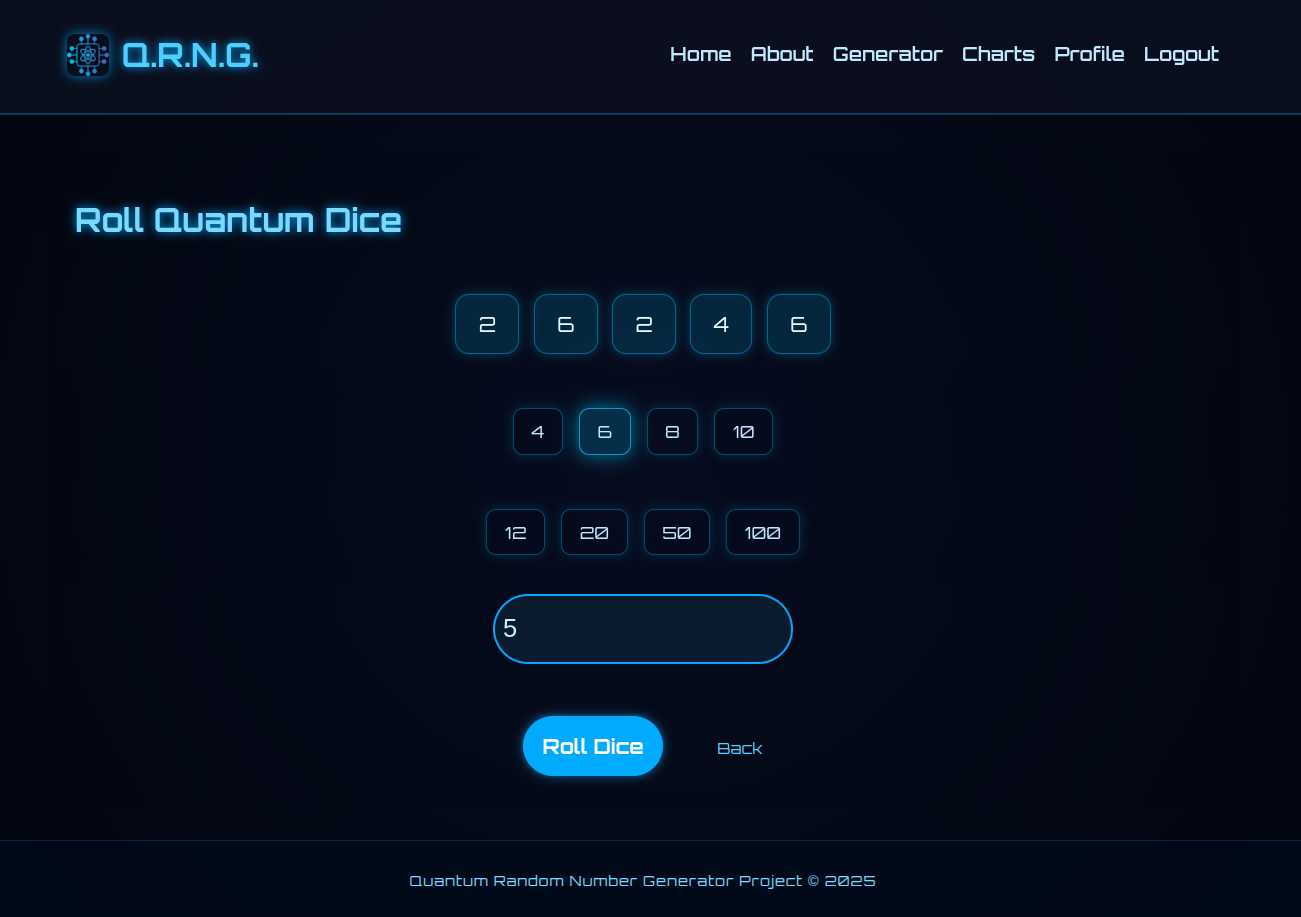
\includegraphics[width=0.8\textwidth]{images/diceRNG}
  \caption{Stránka hodu kockou s výberom typu a výsledkami.}
  \label{fig:dicePage}
\end{figure}

\subsubsection{Všeobecný generátor}

Modul všeobecného generátora (\texttt{/generator/}) poskytuje najuniverzálnejšiu funkcionalitu.
Používateľ zadá dolnú (\texttt{from}) a hornú (\texttt{to}) hranicu intervalu a aplikácia vygeneruje jedno náhodné celé číslo v tomto rozsahu.
Spolu s výsledkom je používateľovi zobrazená aj technická informácia: konkrétne bity použité z databázy, ich počet a index príslušného kvantového merania (shot index), ako je znázornené na obr.~\ref{fig:generatorPage}.

\begin{figure}[H]
  \centering
  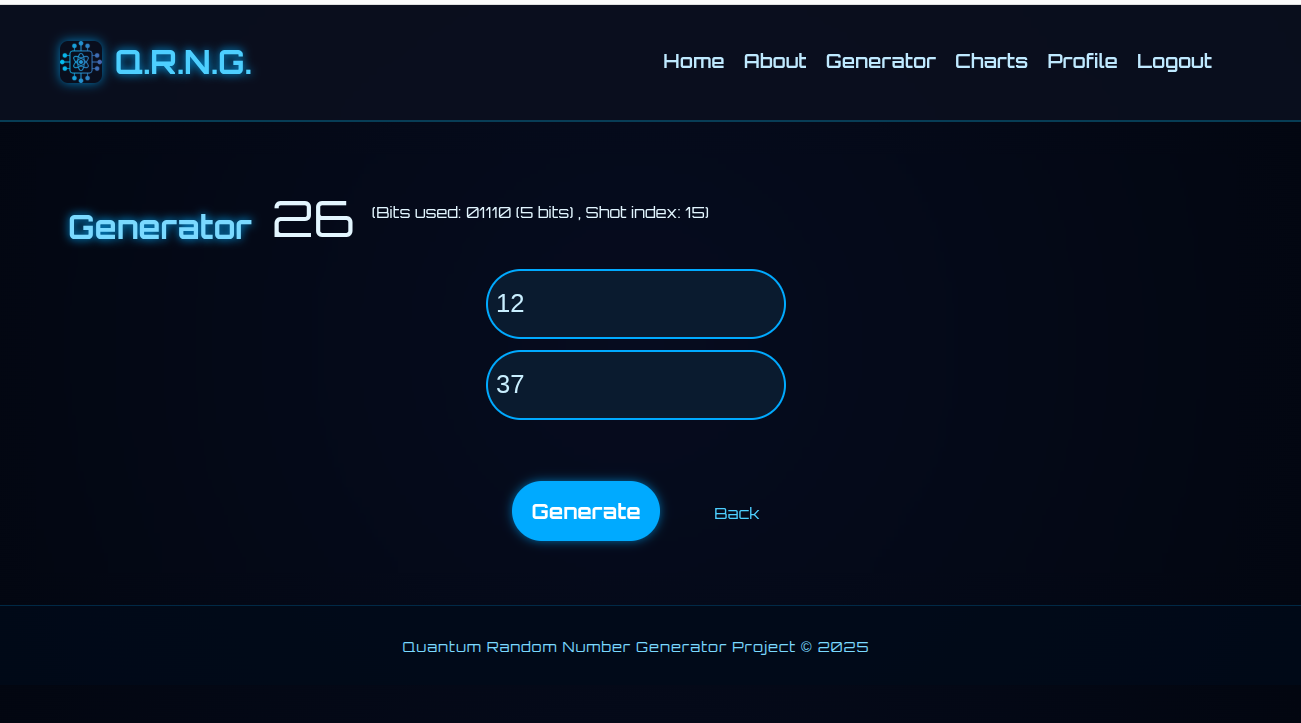
\includegraphics[width=0.9\textwidth]{images/randomNumberGenerator}
  \caption{Všeobecný generátor s výsledkom a detailom použitých bitov.}
  \label{fig:generatorPage}
\end{figure}


\subsection{História generovania}

Pre prihlásených používateľov aplikácia automaticky ukladá každé vygenerované číslo do histórie.
Záznam v tabuľke \texttt{RNGHistory} obsahuje typ generátora (\texttt{coin}, \texttt{dice}, \texttt{generator}), vstupné parametre (napr. typ kocky a počet hodov), samotný výsledok a časovú pečiatku.
Stránka histórie (\texttt{/accounts/history/}), zobrazená na obr.~\ref{fig:historyPage}, zobrazuje záznamy zoradené od najnovšieho s podporou stránkovania -- na každej stránke sa zobrazuje 10 záznamov.
Toto riešenie je priamo integrované do navigačného menu pre prihlásených používateľov a umožňuje im kedykoľvek skontrolovať predchádzajúce výsledky.

\begin{figure}[H]
  \centering
  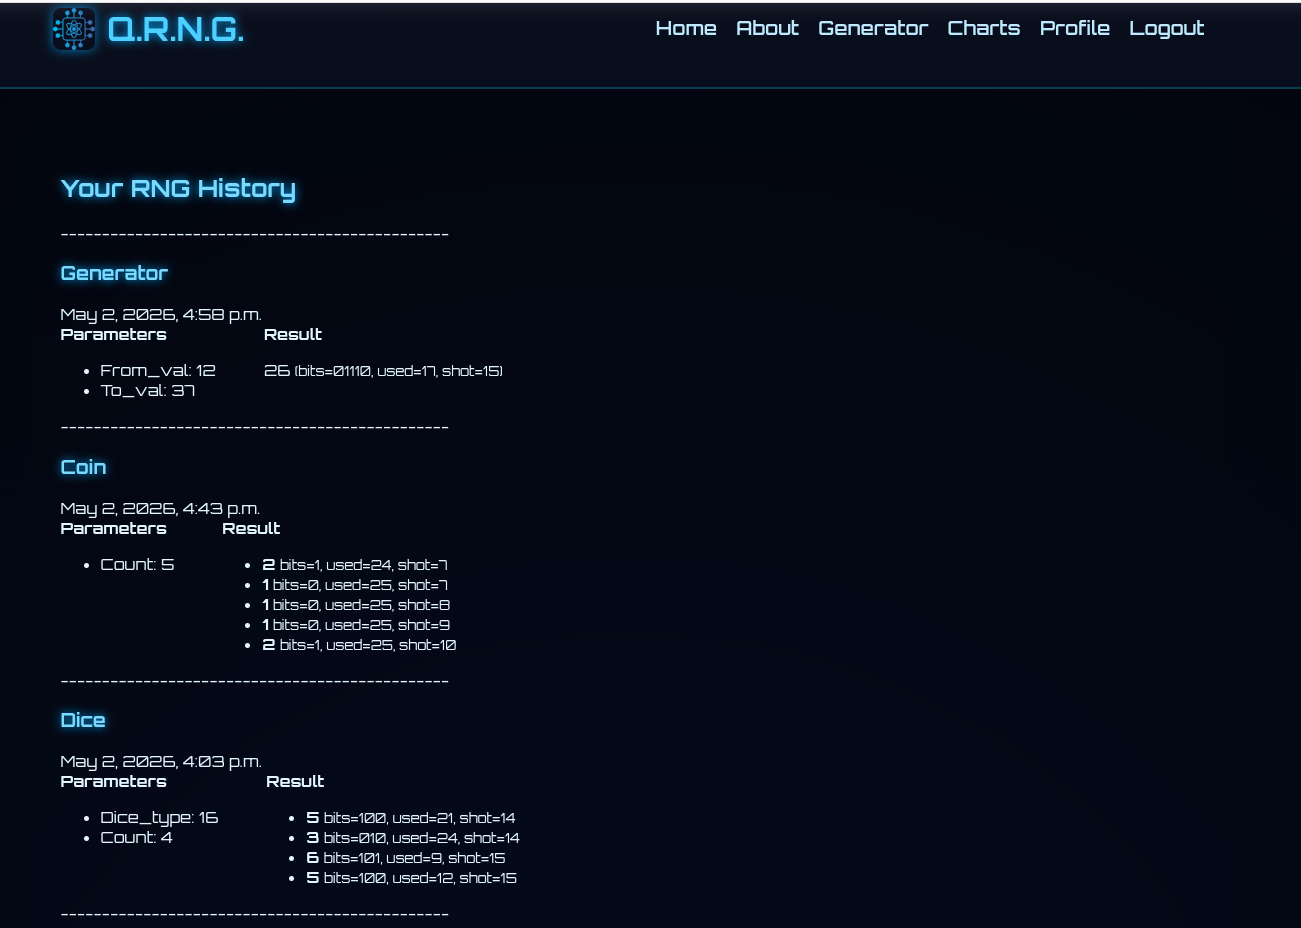
\includegraphics[width=0.9\textwidth]{images/historyRNG}
  \caption{Stránka histórie generovania so záznamami.}
  \label{fig:historyPage}
\end{figure}


\subsection{Profil používateľa}

Každý prihlásený používateľ má prístup k stránke profilu (\texttt{/accounts/profile/}), kde môže upravovať svoje základné údaje (meno, priezvisko, e-mail).
Rozhranie profilu je navrhnuté tak, aby bežným používateľom nezobrazovalo citlivé administrátorské polia: atribúty \texttt{user\_type} a \texttt{token} sú viditeľné a editovateľné iba administrátorom.
Táto ochrana je implementovaná na úrovni serverovej logiky -- ak nie je požadovaná úroveň oprávnení, príslušné polia sú programovo odstránené z formulára ešte pred jeho vykreslením, a zároveň sú pôvodné hodnoty vynútené pri ukladaní, čo zabraňuje ich manipulácii cez priamo odoslaný HTTP POST.
Ukážka stránky profilu je zobrazená na obr.~\ref{fig:profilePage}.

\begin{figure}[H]
  \centering
  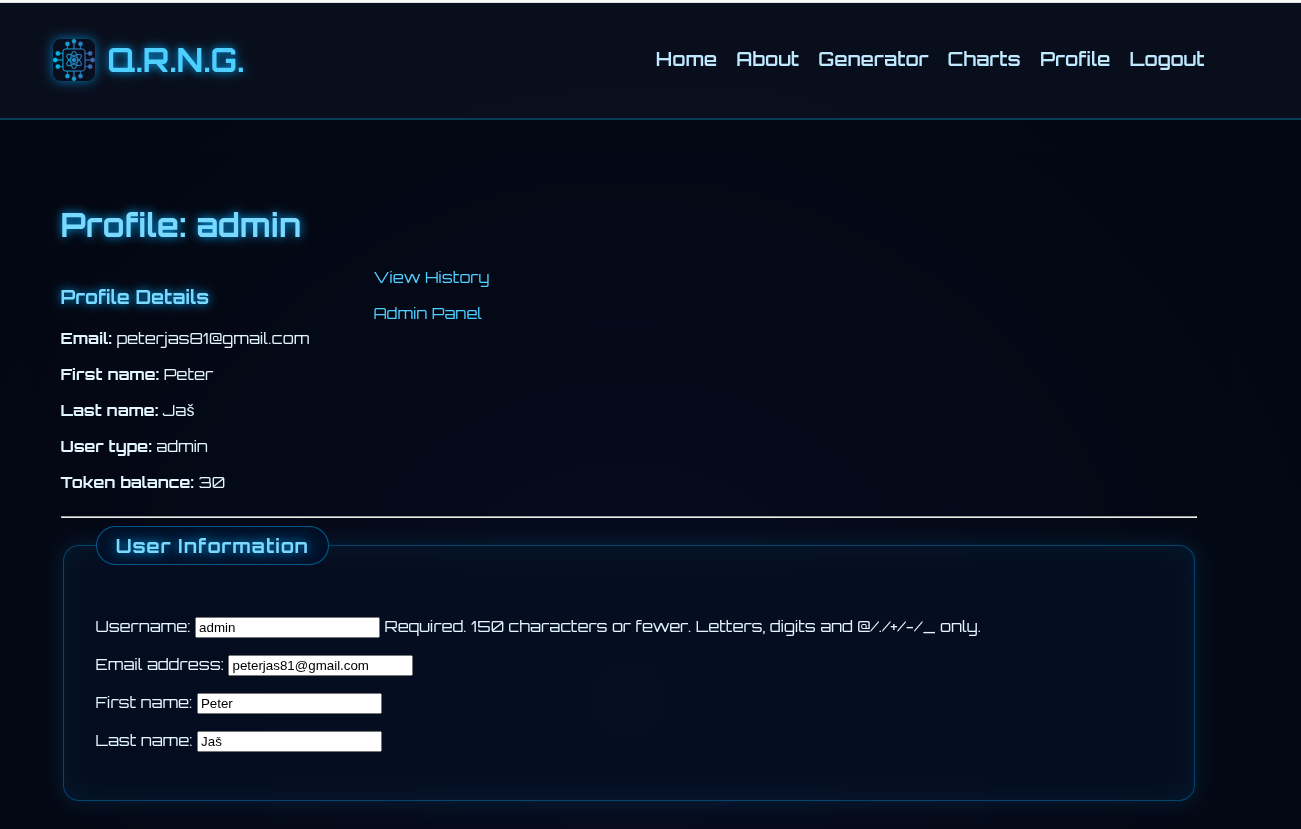
\includegraphics[width=0.9\textwidth]{images/profileRNG}
  \caption{Stránka profilu používateľa.}
  \label{fig:profilePage}
\end{figure}


\subsection{Administrátorské rozhranie}

Administrátorské rozhranie (\texttt{/administration/}) je prístupné výhradne používateľom s typom \texttt{admin}.
Pri pokuse o prístup neoprávneného používateľa aplikácia vráti HTTP odpoveď 403 Forbidden.

Panel administrátora, zobrazený na obr.~\ref{fig:adminPage}, poskytuje prehľad o aktuálnom stave systému v reálnom čase:

\begin{itemize}
  \item \textbf{Počet registrovaných používateľov} -- celkový počet profilov v databáze,
  \item \textbf{Celkový počet dostupných kvantových bitov} -- vypočítaný ako počet záznamov v tabuľke \texttt{QuantumShotResult} vynásobený počtom bitov na záznam (25~bitov),
  \item \textbf{Počet spotrebovaných bitov} -- súčet hodnôt \texttt{used\_bits} zo všetkých záznamov,
  \item \textbf{Zostatok bitov} -- rozdiel medzi celkovým počtom a spotrebovanými bitmi, čo umožňuje sledovať, kedy bude potrebné nahrať nové kvantové dáta.
\end{itemize}

Panel tiež obsahuje akčné tlačidlá.
Prvé umožňuje načítať nové kvantové merania zo súboru \texttt{results1000shot.json} uloženého na serveri -- táto operácia vloží nové záznamy do databázy a aktualizuje dostupné bity.
Druhé tlačidlo presmeruje administrátora na správu používateľov.
Tretie tlačidlo vykoná reset databázy kvantových meraní nastavením hodnoty \texttt{used\_bits} na 0 pre všetky záznamy, čím sa efektívne obnoví celý zásobník náhodnosti bez nutnosti opätovného nahrávania dát.

\begin{figure}[H]
  \centering
  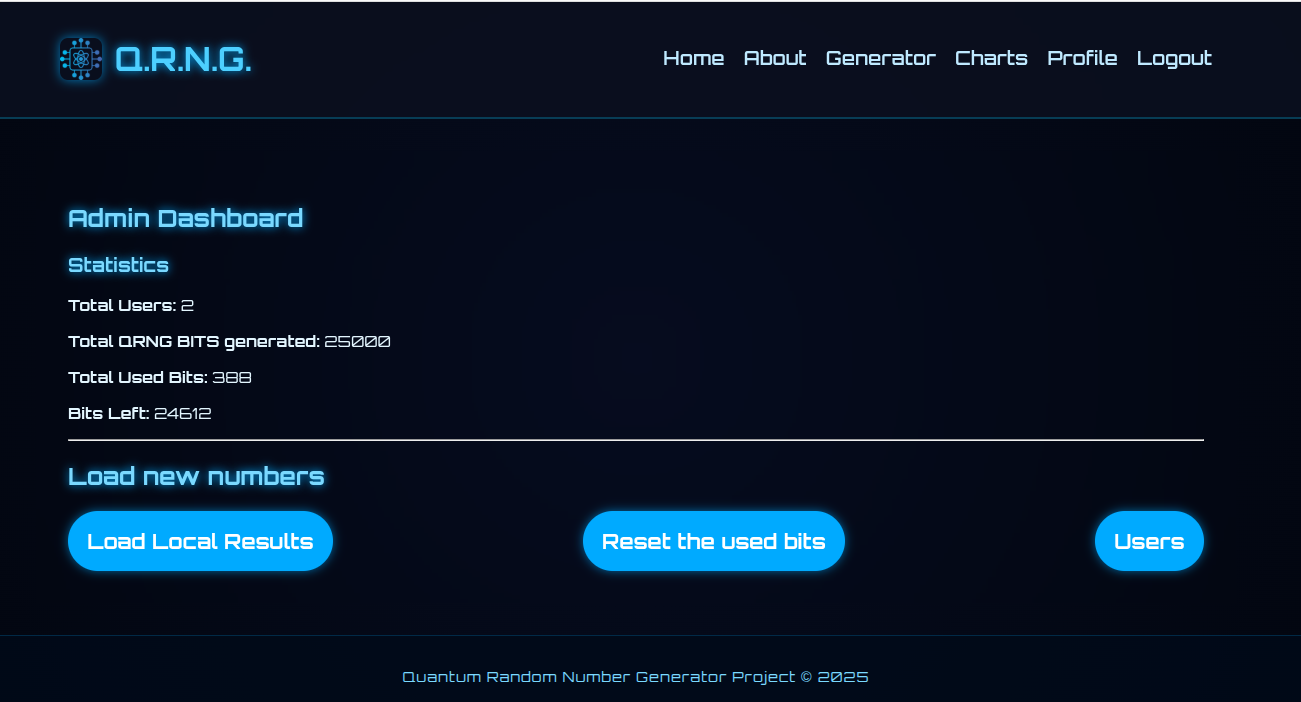
\includegraphics[width=0.9\textwidth]{images/adminRNG}
  \caption{Administrátorský panel so štatistikami systému.}
  \label{fig:adminPage}
\end{figure}


\subsection{Správa používateľov}

Administrátor má k dispozícii aj stránku správy používateľov (\texttt{/accounts/users/}), kde vidí zoznam všetkých registrovaných účtov vrátane ich používateľského mena, e-mailovej adresy, typu účtu a tokenu.
Pre každého používateľa môže priamo z tejto stránky zmeniť hodnotu \texttt{user\_type} (napr. povýšiť bežného používateľa na administrátora) a upraviť hodnotu \texttt{token}.
Stránka je dostupná z administrátorského panelu aj priamou URL adresou, pričom prístup je chránený rovnakým overením oprávnení ako samotný panel.



\section{Diskusia a prínosy práce}


Na základe vyhodnotenia možno konštatovať, že navrhnutý kvantový generátor náhodných čísel:


\begin{itemize}

  \item produkuje bitové sekvencie s vysokou mierou náhodnosti,

  \item vykazuje stabilné štatistické vlastnosti,

  \item spĺňa základné požiadavky kryptografickej bezpečnosti,

  \item efektívne využíva kvantové javy ako zdroj náhodnosti.

\end{itemize}


Zároveň sa ukázalo, že kvalita výstupu je ovplyvnená fyzikálnymi obmedzeniami kvantového hardvéru, ako sú šum, decoherencia a chybovosť merania.
Použitie extrakcie entropie však tieto nedostatky výrazne redukuje.

Výsledky práce potvrdzujú, že kvantové generátory predstavujú perspektívny zdroj kvalitnej náhodnosti,
ktorý môže byť využitý najmä v oblasti kryptografie a bezpečnostných aplikácií.
